\documentclass{beamer}
\usetheme{Warsaw}

\usepackage[utf8]{inputenc}
\usepackage{fancybox}
\usepackage{multimedia} 
\usepackage{subfig}
\usepackage{amsmath}

\usepackage[all]{xy}
\begin{document}


\title[Computergrafik] % (optional, only for long titles)
{Computergrafik

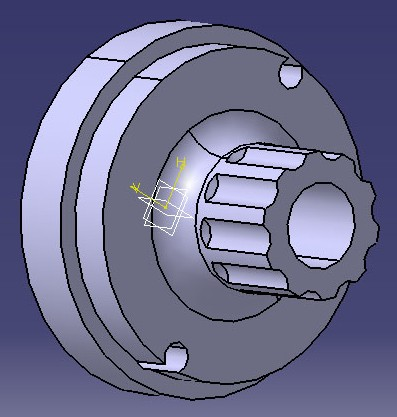
\includegraphics[scale=0.36]{images/CAD3D}
}
\subtitle{}
\author[Dr. Johannes Riesterer] % (optional, for multiple authors)
{Dr.  rer. nat. Johannes Riesterer}

\date[KPT 2004] % (optional)
{}

\subject{Computergrafik}

\begin{frame}
    \frametitle{CAD}
\framesubtitle{}
    \begin{block}{Computer Aided Design}
\begin{center}
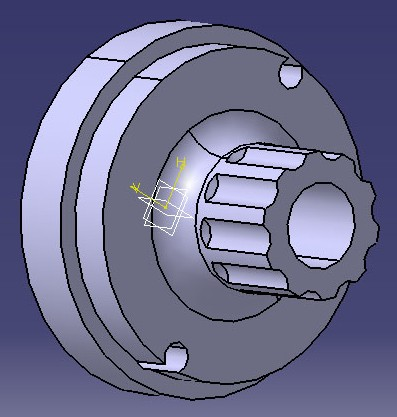
\includegraphics[scale=0.45]{images/CAD3D}
\end{center}
\end{block}

\end{frame}



\begin{frame}
    \frametitle{CAD}
\framesubtitle{}
    \begin{block}{FreeCAD}
\begin{center}
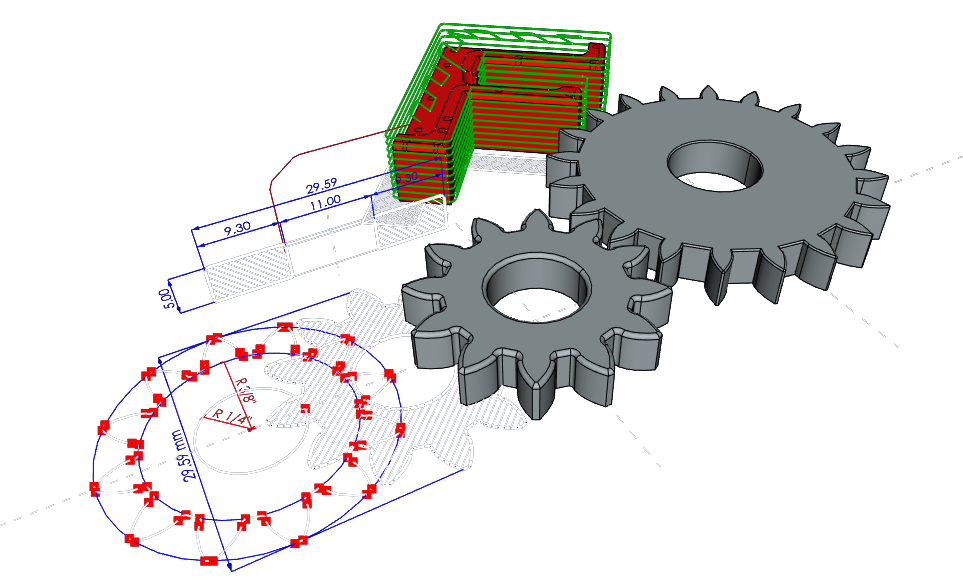
\includegraphics[scale=0.25]{images/freecad}
\end{center}
\end{block}

\begin{block}{Link}
\href{https://www.freecadweb.org/}{FreeCAD} \\
\href{https://wiki.freecadweb.org/Tutorials/}{FreeCAD Tutorials}

\end{block}

\end{frame}



\begin{frame}
    \frametitle{CAD}
\framesubtitle{}
    \begin{block}{Openscad}
\begin{center}
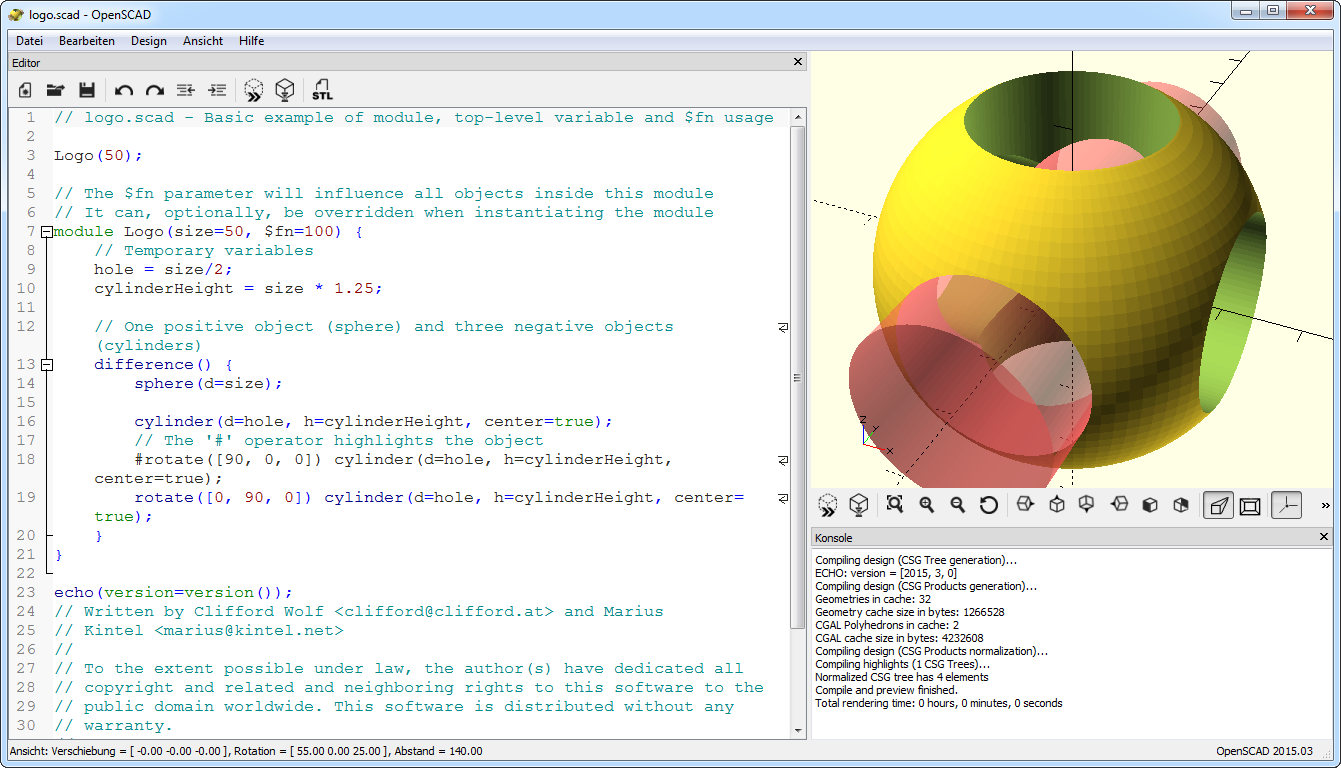
\includegraphics[scale=0.15]{images/Openscad}
\end{center}
\end{block}

\begin{block}{Link}
\href{https://openscad.org/}{OpenSCAD}


\end{block}

\end{frame}


\begin{frame}
    \frametitle{CAD}
\framesubtitle{}
    \begin{block}{Modellierkern}
\begin{center}
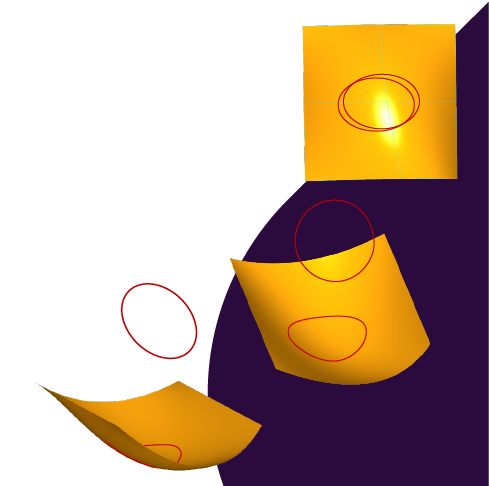
\includegraphics[scale=0.25]{images/kern}
\end{center}
\end{block}

\begin{block}{Link}
\href{https://de.wikipedia.org/wiki/Modellierkern}{Modellierkern}
\end{block}

\end{frame}

\begin{frame}
    \frametitle{CAD}
\framesubtitle{}
    \begin{block}{BRB}
\begin{center}
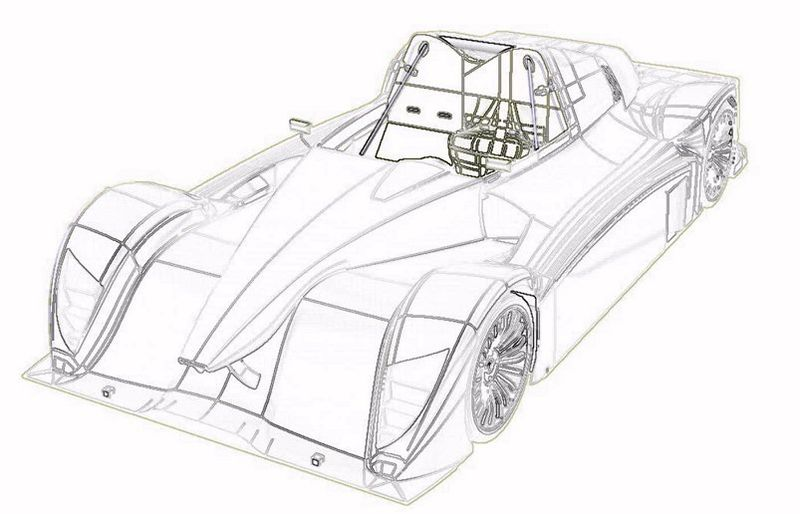
\includegraphics[scale=0.85]{images/brb}
\end{center}
\end{block}

\begin{block}{Link}
\href{https://de.wikipedia.org/wiki/Boundary_Representation}{Begrenzungsflächenmodell (BRep)}
\end{block}

\end{frame}






\begin{frame}{Modellierung}
\frametitle{Bezier Kurven und Flächen}
\framesubtitle{}
 \begin{block}{Bernsteinpolynome}
Die Bernsteinpolynome vom Grad $n$ sind definiert als
\begin{align*}
\framesubtitle{}
B_i^n(t) := \begin{pmatrix} n \\ i \end{pmatrix} (1-t)^{n-i}t^i
\end{align*}
mit $i = 0, \hdots n$, $t \in [0,1]$ und dem Binomialkoeffizient
\begin{align*}
\begin{pmatrix} n \\ i \end{pmatrix} := \frac{n!}{i!(n-i)!} = \frac{n(n-1) \cdots 1}{i(i-1) \cdots 1 (n-i) (n-i-1) \cdots 1 } \; .
\end{align*}
\begin{align*}
\begin{pmatrix} n \\ i \end{pmatrix} = \begin{pmatrix} n-1 \\ i \end{pmatrix} + \begin{pmatrix} n-1 \\ i-1 \end{pmatrix} 
\end{align*}
\end{block}

\end{frame}


\begin{frame}{Modellierung}
\frametitle{Bezier Kurven und Flächen}
\framesubtitle{}

\begin{center}
    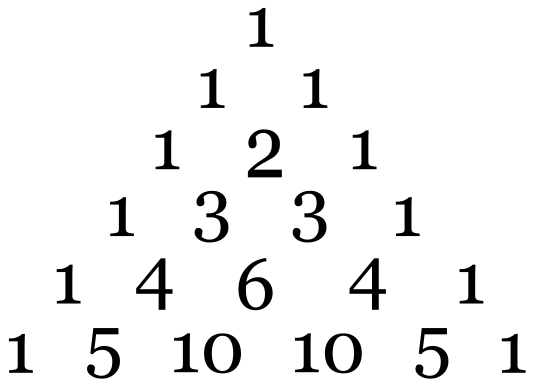
\includegraphics[scale=0.2]{images/pascal.png}

    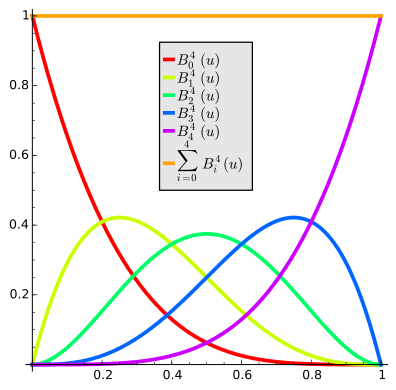
\includegraphics[scale=0.45]{images/Bernstein_Polynomials.png}
\end{center}
\end{frame}


\begin{frame}{Modellierung}
\frametitle{Bezier Kurven und Flächen}
\framesubtitle{}
 \begin{block}{Bernsteinpolynome}

Die Bernsteinpolynome vom Grad $n$ bilden eine Basis des Vektorraums der Polynome vom Grad $n$ im Intervall $[0,1]$.
\end{block}

 \begin{block}{Bernsteinpolynome}
Es gilt die Rekursionsformel
\begin{align*}
B_i^n(t) = (1-t) \cdot B^{n-1}_{i}(t) + t \cdot B^{n-1}_{i-1}(t)
\end{align*}
mit $B^0_0(t) = 1$ und $B^i_n(t) = 0$ für $i<0$ oder $i>n$.
\end{block}


Folgt fast direkt aus der Rekursionsformel des Binomialkoeffizienten.

\end{frame}

\begin{frame}{Modellierung}
\frametitle{Bezier Kurven und Flächen}
\framesubtitle{}
 \begin{block}{Bernsteinpolynome}
Seien $b_0, \hdots b_n \in \mathbb{R}^3$. Dann heißt die Kurve
\begin{align*}
B^n(t) := \sum_{i = 0}^{n} B_i^n(t) \cdot  b_i \; , t \in [0,1] 
\end{align*} 
eine Bezierkurve vom Grad $n$. Die $b_i$ werden auch Kontrollpunkte genannt.
Für ein beliebiges Intervall $[a,b]$ definieren wir
\begin{align*}
B^n_{[a,b]} (t):=  B^n\biggl( \frac{t-a }{a-b} \biggr) \; , t \in [a,b] \; .
\end{align*} 
\end{block}
\end{frame}

\begin{frame}{Modellierung}
\frametitle{Bezier Kurven und Flächen}
\framesubtitle{}
 \begin{block}{Bernsteinpolynome}
Eine Bezierkurve hat die Ableitung
\begin{itemize}
\item $(B^n)'(t) = n \cdot \sum_{j = 0}^{n-1} B_{j}^{n-1}(t) \cdot (b_{j+1} - b_j) \; ,$ und nach der Kettenregel
\item $(B^n_{[a,b]})'(t) = \frac{1}{b-a} (B^n)' \bigl(\frac{t -a}{b-a} \bigr)$  für ein beliebiges Parameterintervall.
\end{itemize}
\end{block}


\end{frame}





\begin{frame}{Modellierung}
\frametitle{Bezier Kurven und Flächen}
\framesubtitle{}

  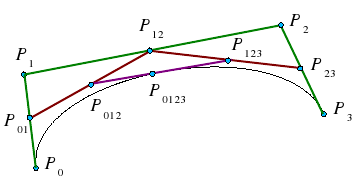
\includegraphics{images/decasteljau}

Sei $B^n(t) := \sum_{i = 0}^{n} B_i^n(t) \cdot  b_i$ eine Bezierkurve. Für ein 
$t_0 \in [0,1]$ definieren wir rekursiv  
\begin{align*}
b_i^k := \begin{cases}
b_i   & i= 0, \hdots,  n \\
(1-t_0) \cdot b_{i-1}^{k-1} + t_0 \cdot b_{i}^{k-1} &  i = 1, \hdots , n \; \;   k = 1, \hdots , i 
\end{cases} 
\end{align*}
\end{frame}


\begin{frame}{Modellierung}
\frametitle{Bezier Kurven und Flächen}
\framesubtitle{}


\begin{align*}
\xymatrix{
b_0   \ar@{}[r]|-{=}  &  b_0^0 \ar[dr]^{\cdot(1-t_0)}  &  & & & & & &  \\
b_1   \ar@{}[r]|-{=}  &  b_1^0  \ar[r]^{\cdot t_0} \ar[dr]^{\cdot(1-t_0)} &   b_1^1  \ar[dr]^{\cdot(1-t_0)} & & & & & & \\
b_2   \ar@{}[r]|-{=}  \ar@{..}[d] &  b_2^0  \ar[r]^{\cdot t_0}  \ar@{..}[d] &   b_2^1 \ar[r]^{\cdot t_0}  \ar@{..}[d] &  b_2^2   \ar@{..}[dr]& & & & & \\
b_{n-1}   \ar@{}[r]|-{=}  &  b_{n-1}^0   \ar[r]^{\cdot t_0}  \ar[dr]^{\cdot(1-t_0)} &    b_{n-1}^1   \ar[r]^{\cdot t_0}  \ar[dr]^{\cdot(1-t_0)} &  b_{n-1}^2  \ar@{..}[r] &  
b_{n-1}^{n-1}  \ar[dr]^{\cdot(1-t_0)} & & & & \\
b_{n}   \ar@{}[r]|-{=}  &  b_{n}^0  \ar[r]^{\cdot t_0}  &    b_{n}^1   \ar[r]^{\cdot t_0}  &  b_{n}^2  \ar@{..}[r] & b_{n}^{n-1}   \ar[r]^{\cdot t_0}& b_{n}^{n}& & & 
}
\end{align*}
Dann gilt $b_n^n = B^n(t_0)$.

\end{frame}

%\begin{frame}{Modellierung}
%\frametitle{Bezier Kurven und Flächen}
%\framesubtitle{}

%Seien $B^n(t)$ und $(B^*)^m(t)$  Bezierkurven. Man spricht von einem $C^0$-Patching (an der Stelle $B^n(1)$), falls
% $B^n(1) = (B^*)^m(0) $ gilt. Stimmen auch die Ableitungen überein, also  $(B^n)'(1) = ((B^*)^m)'(0) $, dann spricht man von einem $C^1$-Patching und stimmen noch für $k> 1$ auch
%die höheren Ableitungen $(B^n)^{k}(1) = ((B^*)^m){k}(0) $ überein, so spricht man von einem $C^k$-Patching . 



%Zwei Bezierkurven   $B^n(t) := \sum_{i = 0}^{n} B_i^n(t) \cdot  b_i$ und $(B^*)^m(t) := \sum_{i = 0}^{m} B_i^n(t) \cdot  b^*_i$ bilden genau dann einen $C^1$-Patch  (an der Stelle $B^n(1)$), wenn 
%$B^n(1) = (B^*)^m(0)$ und $\Bigl(B^n(1) - b_{n-1} \Bigr)= - \frac{m}{n}  \Bigl((B^*)^m(0) - (b^*)_1 \Bigr)$ gilt.


%Ist  $B^n(t)$ eine Bezierkurve, so bilden die Bezierkurven $(B^{*})^n(t)  :=  \sum_{i = 0}^{n} B_i^n(t/2) \cdot  b_i^i$ und  $(B^{**})^n(t)  :=  \sum_{i = 0}^{n} B_i^n( \frac{t+1} {2}) \cdot  b_n^{n-i}$
%einen $C^1$-Patch.

%\end{frame}


\begin{frame}{Modellierung}
\frametitle{Bezier Kurven und Flächen}
\framesubtitle{}

Ersetzt man in einer Bezierkurve 
\begin{align*}
B^m(v) := \sum_{j = 0}^{m} B_j^m(v) \cdot  b_j
\end{align*}
vom Grad $m$ die Kontrollpunkte $b_j$ durch $m+1$ Bezierkurven
\begin{align*}
b_j (u)= \sum_{i = 0}^{n} B_i^n(u) \cdot  b_{ij}
\end{align*}
 vom Grad $n$ mit jeweils $n+1$ Kontrollpunkten $ b_{ij}$ für $i = 0, \cdots , n$, so erhält man eine Fläche
\begin{align*}
F(u,v) =  \sum_{i = 0}^{n}  \sum_{j = 0}^{m} B_i^n(u) B_j^m(v) \cdot  b_{ij} \; ,
\end{align*}
welche auch Tenorprodukt-Fläche der Bezierkurven  oder einfach Bezierfläche genannt wird.


\end{frame}


\end{document}
